\documentclass[letterpaper,12pt]{article}

\usepackage{mathpazo}
\usepackage[longnamesfirst]{natbib}
\usepackage[flushleft]{threeparttable} 
\usepackage{booktabs}
\usepackage{rotating} 
\usepackage{amssymb} 
\usepackage{amsmath}
\usepackage{caption} 
\usepackage{dcolumn} 
\usepackage{setspace}
\usepackage[longnamesfirst]{natbib}
\usepackage[font=scriptsize]{subfig}
\usepackage[pdftex,colorlinks=true,linkcolor=black,citecolor=black]{hyperref} 
\usepackage[margin=1.0in]{geometry} 
\usepackage{multirow}

\newcommand{\mco}[1]{\multicolumn{1}{c}{#1}}
\newcommand{\mct}[1]{\multicolumn{2}{c}{#1}}


%opening
\title{Fertility Issues in Developing Countries} 

\author{Claus C P\"ortner\\
    Department of Economics\\
    Albers School of Business and Economics\\
    Seattle University, P.O. Box 222000\\
    Seattle, WA 98122\\
    \href{mailto:cportner@seattleu.edu}{\texttt{cportner@seattleu.edu}}\\
    \href{http://www.clausportner.com}{\texttt{www.clausportner.com}}\\
    \& \\
    Center for Studies in Demography and Ecology \\
    University of Washington\\ \vspace{2cm}
    }

\date{February 2017}

\doublespacing

\begin{document}
\graphicspath{{../figures/}}
\DeclareGraphicsExtensions{.jpg,.jpeg,.pdf,.mps,.png}

\maketitle
\thispagestyle{empty}


\newpage

\section{Introduction}

Despite a common perception that fertility is very high in developing countries,
the truth is substantially more complicated.
Figure \ref{fig:TFR} shows that there has been an astonishing decline in 
most developing countries' total fertility rate (TFR) over the last half 
century.%
\footnote{
TFR is the number of children a women entering her reproductive life
would have if she had children following the age-specific fertility
rates observed at that point in time.
Hence, it is composite or snapshot measure of current fertility
behavior.
}
Half a decade ago, TFR was around 7 children, with the exception
of Europe and Central Asia.
The most recent data show, however, that, with the exception of 
Sub-Saharan African, TFR is now either below or only slightly 
above the replacement level of 2.1.
Despite this rapid decline in fertility population size is still
growing in many of these regions because there are still many
more young people than older people and these young people either
have not entered reproductive age or are just starting out.

\begin{figure}[hp]
    \centering
    \caption{Total Fertility Rates by Region from 1967 to 2015}
    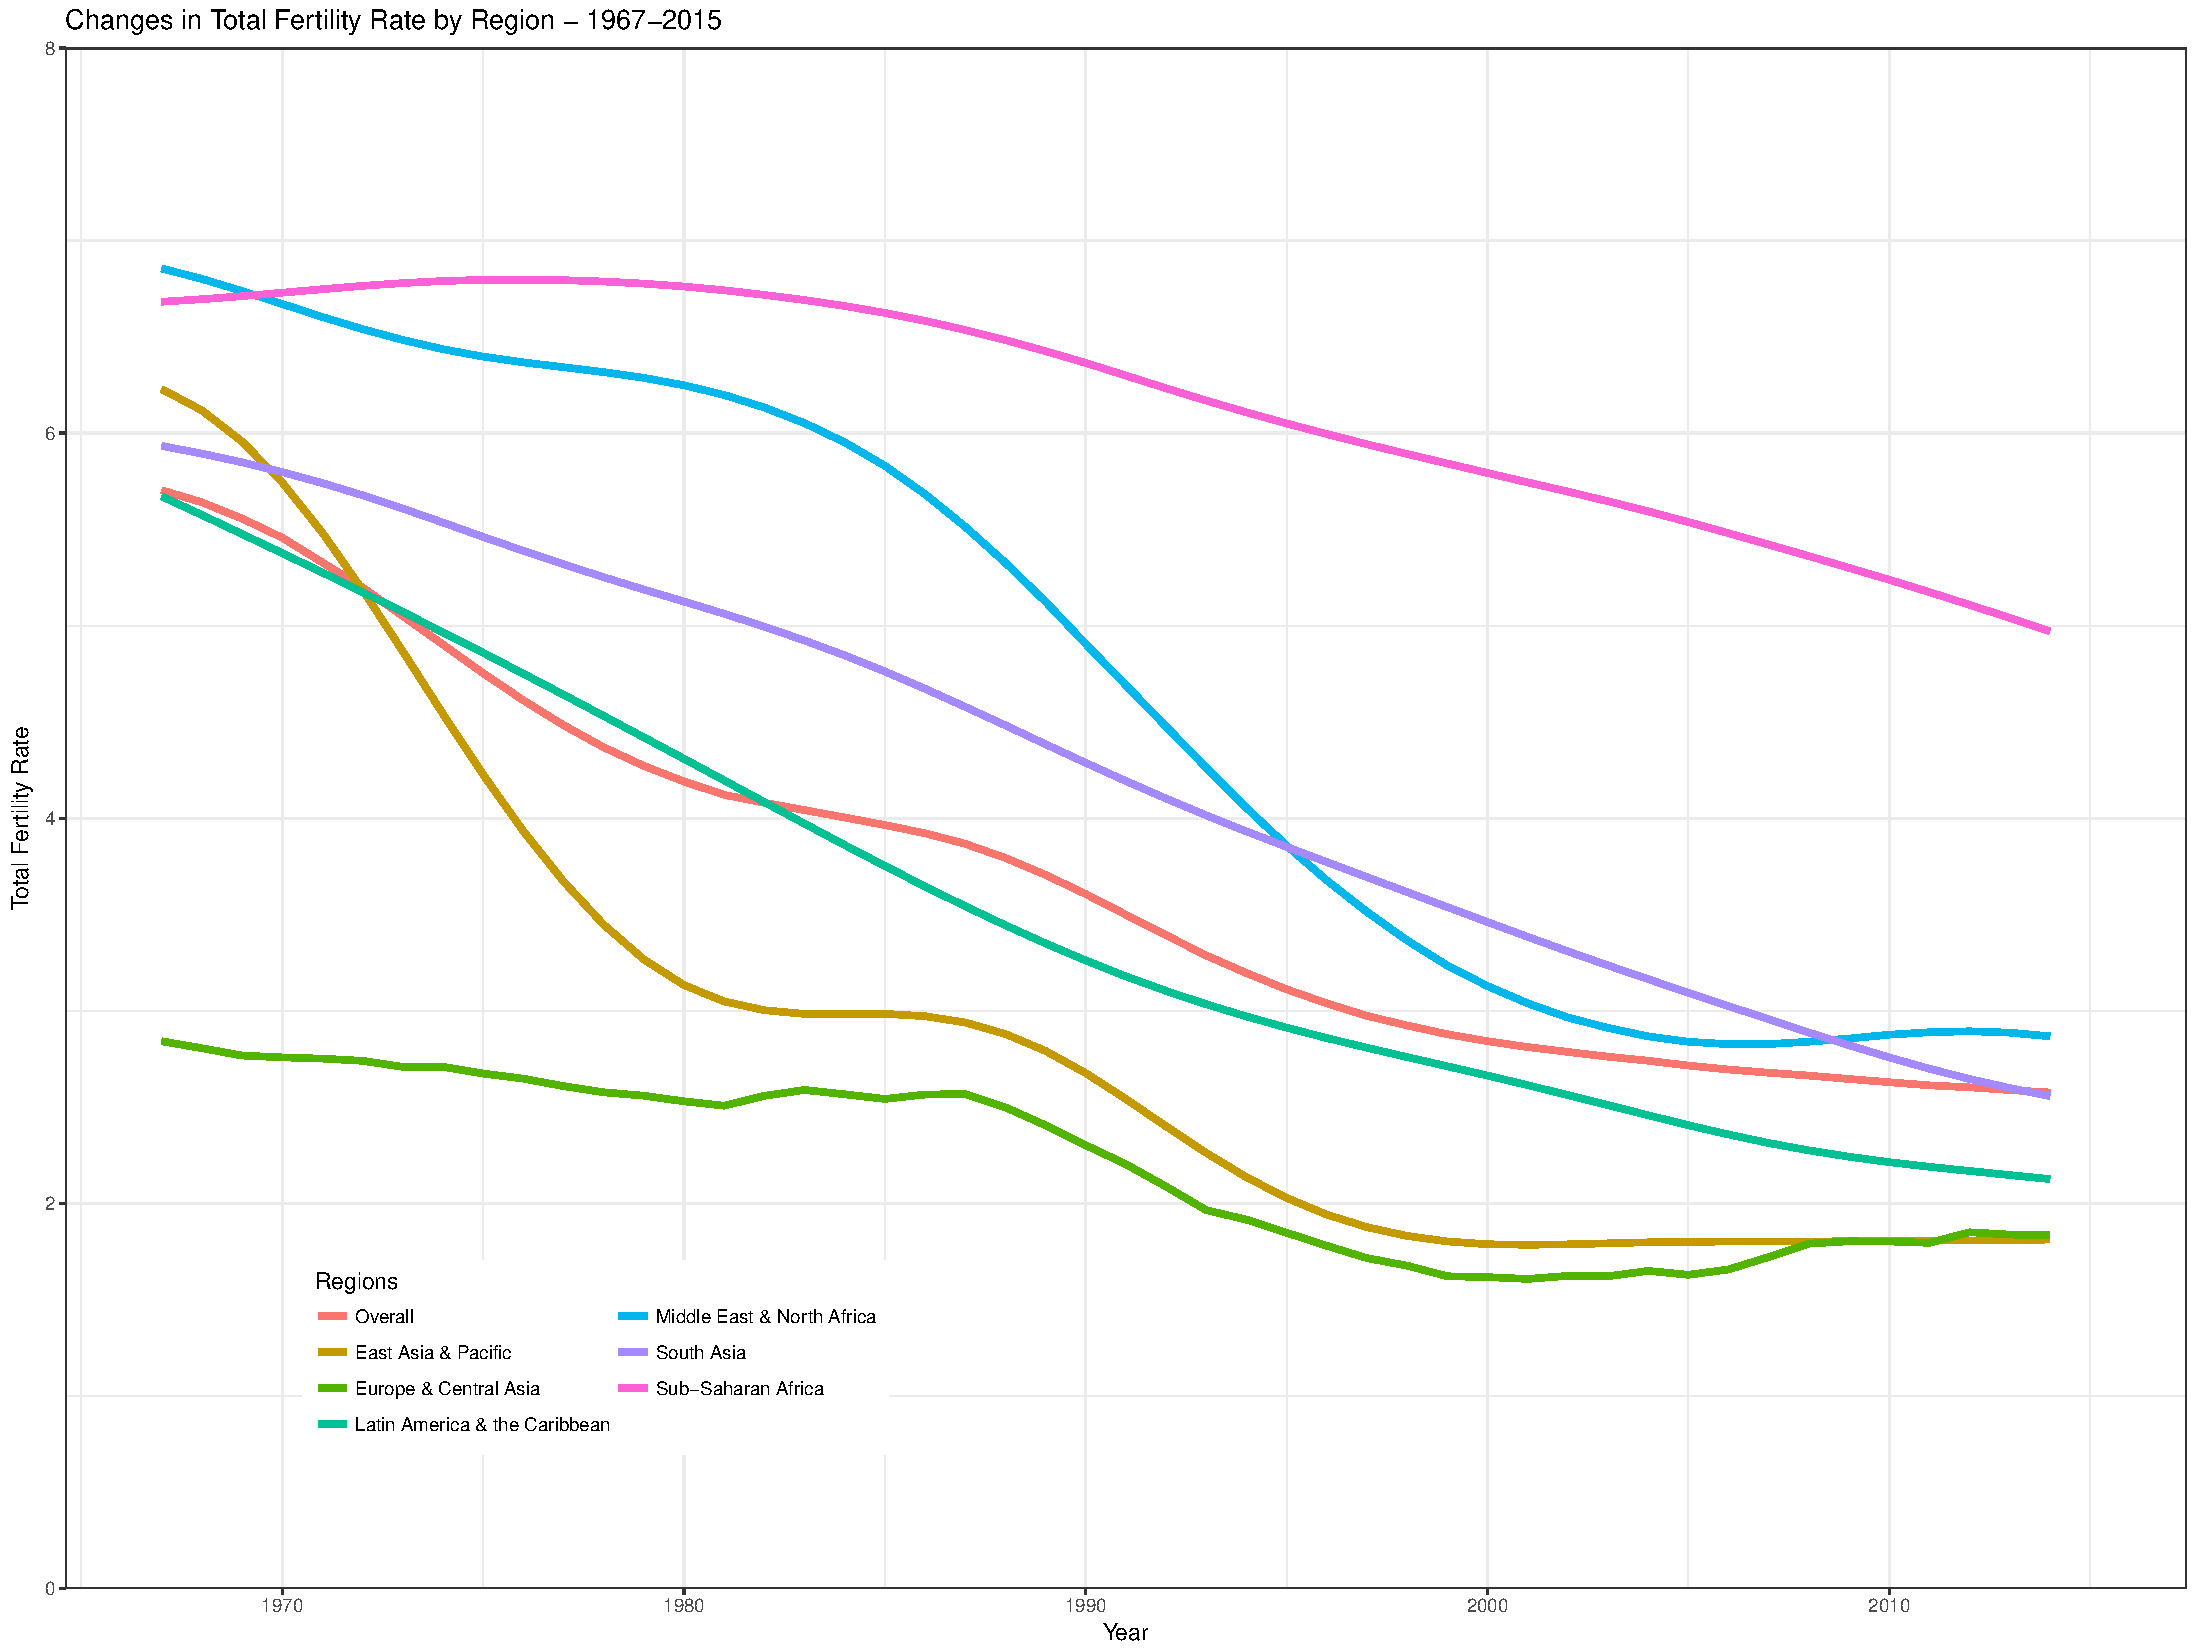
\includegraphics[width=0.75\linewidth]{totalFertilityRates}
    \label{fig:TFR}
\end{figure}

If fertility levels are close to identical across developing and
developed countries and there is rapid urbanization and increasing
labor force participation among women do we even need a developing 
country version of this chapter?%
\footnote{
TK references on urbanization and labor force particpation.
}
The goal of this chapter is to highlight the areas in which a
separate focus on developing countries is still relevant,
what the recent developments in research has been, and
most importantly, what I consider to be the main
outstanding issues.

[still need policy discussion; this seems kind of a rambling list]
Furthermore, we still know relatively little about determinants
of timing of births in developing countries.
People in most developing countries are also still subject to
higher risk of shocks, be that from weather, health, or political,
but we still have little idea of how people respond to the level
of risk and the occurrence of shocks.
Finally, both in developed and developing countries we have
mostly treated fertility decisions as separate from other
household decision and preferences [ehh, Becker theory!].
We still need to know more about how husband and wife decides
on fertility if they are have different preferences 
and how allocation decisions across all household member are
related to fertility decisions.
A prime example that I will treat separately is the role
of son preferences in fertility decisions.




\section{Sub-Saharan Africa}

The outlier in the figure above is Sub-Saharan Africa. 
Sub-Saharan Africa now has an average TFR that is about twice
as large as the other regions.
Most of the projected future increase in world population 
is therefore likely to come from Sub-Saharan Africa 
\citep{Gerland2014}.%
\footnote{
Currently Africa is home to about 1 billion people, but this
will increase to between 3.1 and 5.7 billion by the end of
the century.
}
The most important issues from a policy standpoint is why the 
fertility decline in Sub-Saharan Africa have moved at a much
slower pace than the other regions and even appears to
have stalled in some countries \citep{Ainsworth1996a,Singh2017}.
The purpose of this section is not to provide the final answer, but
instead to highlight both how we can think about fertility
decisions and suggest possible answers.

Broadly speaking there are two competing approaches to 
explaining fertility decisions.%
\footnote{
This is clearly a simplification but it serves to illustrate
the differences in approaches.
}
One sees fertility preferences as the main driver of fertility and
considers preferences malleable and mainly determined by cultural 
factors and transmission of ideas of ideal family size across groups.
Under this approach the main constraints on reaching desired 
fertility is the level of access to family planning and 
contraceptives.

The other sees the decision on fertility as driven by the
trade-off between the cost of children and the return to children,
which can either be monetary or the utility of having offspring.
In this approach parents are assumed to be able to control 
fertility even in the absence of modern contraceptives.
Hence, although lower cost of preventing births---for example
easier access to modern contreceptive---will still lower
fertility in this approach the decline in fertility is 
assumed to be much smaller than the first theory.

Both theories consider the surviving number of children as
the main outcome that people are interested in.
One possible explanation for the slow decline in fertility
could therefore be that mortality in Sub-Saharan Africa is
higher than in the other regions.
Figure \ref{fig:mortality} shows the development over time in 
under-5 mortality across the same regions as above.
The improvements in mortality risk over time are truly astonishing.
Over the last half-decade under-5 mortality in developing countries 
has fallen from close to 175 to below 50 per 1,000 live births.
Sub-Saharan Africa, however, lacks substantially behind other regions.
Despite a massive improvement from a situation where more than a
quarter of all children born did not live to see their fifth
birthday to about 80 deaths per 1,000 births, the current mortality 
rate is still more than three times larger than that of the other 
regions (with the exception of Middle East and North Africa).
Although mortality is likely part of the explanation it cannot
be the full explanation.
Mortality in Sub-Saharan Africa is at the same level as it was
in South Asia around the turn of the century, but fertility
is about 1.5 child higher in Sub-Saharan Africa than it was
in South Asia at the turn of the century (and therefore at the
same level of mortality).

\begin{figure}[hp]
    \centering
    \caption{Under-5 Mortality Rates by Region from 1967 to 2015}
    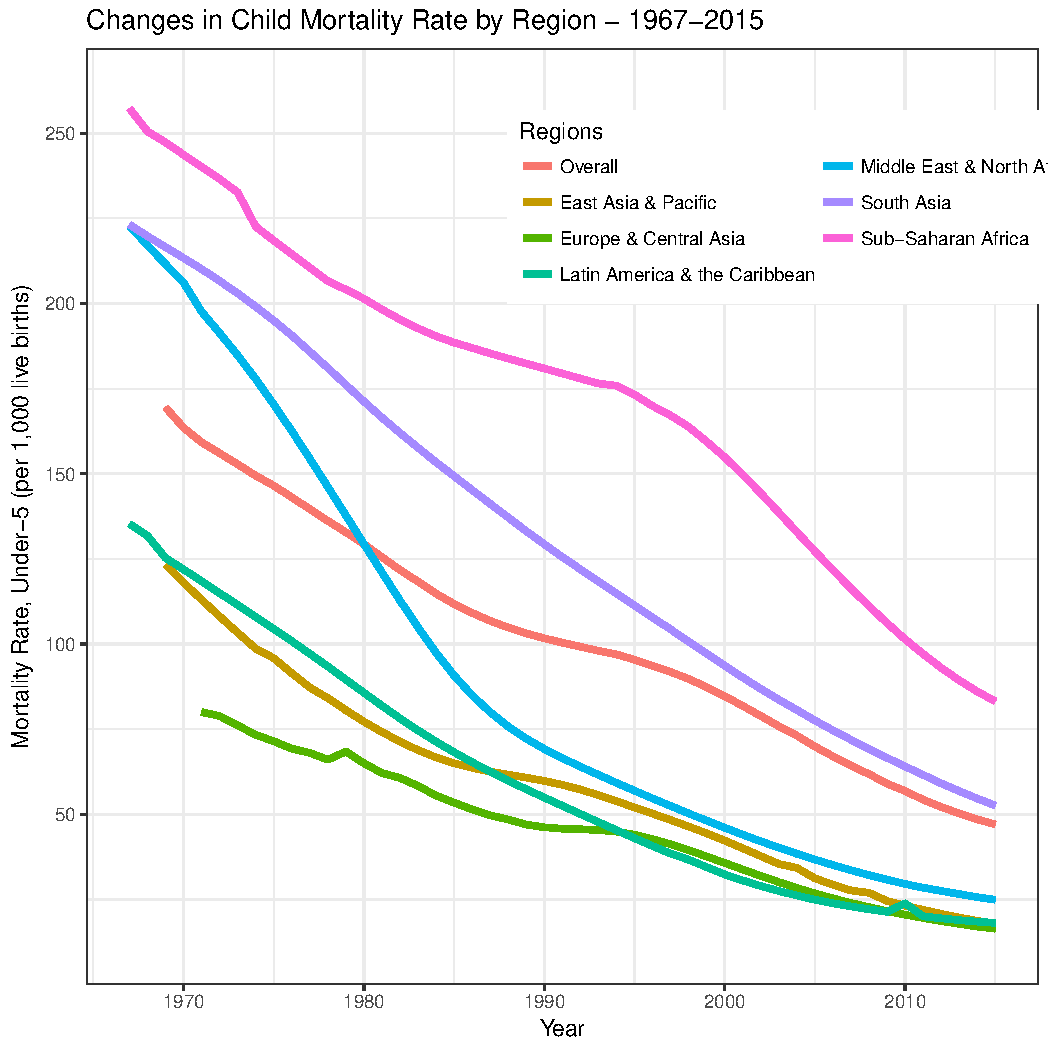
\includegraphics[width=0.75\linewidth]{childMortalityRates}
    \label{fig:mortality}
\end{figure}

If mortality is not the explanation, what might lead to the
higher fertility in Sub-Saharan Africa?
Demographers, following the first approach described above, 
have argued that the two main reasons for the slow decline 
in fertility in Sub-Saharan Africa are the high ideal family 
size still in place and a substantial ``unmet need'' for contraception  
\citep{Bongaarts2013a,Singh2017}.
Contraceptive use is, indeed, lower in Sub-Saharan Africa than
the other regions, but other regions managed to reduced fertility
even in the absence of access to modern contraceptives 
\citet{Schultz1985,Galloway1987,Bailey1998,bengtsson06}.
Furthermore, one difference in fertility behavior between 
Sub-Saharan Africa and the other regions are that the longer 
birth intervals even in the absence of access to modern 
contraception, which are the result of postpartum sexual 
abstinence and extended periods of breastfeeding \citep{Caldwell1992}.
To the extend that the longer birth intervals are the result
of conscious decisions it shows that people are able to
control fertility.%
\footnote{
It is still possible that fertility is higher than desired
because the higher cost of preventing ``accidental''
conceptions.
This would explain why the estimated effect of access to 
family planning in Ethiopia shows a reduction in fertility
of about one birth, which is equivalent to an approximate
20\% reduction in fertility \citet{Portner2014a}.
}


There are three alternative explanation that may explain the
slow decline.
First, the relative abundance of land compared to other regions.
Second, low levels of education; or at least low levels of quality
in education.
Finally, the role of urbanization across regions.  

The effect of land access on fertility works in a couple of 
different way.
First, there is more land per capita in Sub-Saharan Africa than
in the other regions.
At the median projected population growth for Sub-Saharan 
Africa---which is 4.2 billion people by 2100---the 
population density will only be roughly equal to
that of China today \citep[p 235]{Gerland2014}.
The low density means that there is little pressure to 
restrain fertility for fear of running out of land.
In fact, it is likely that there is a higher return to
children in Sub-Saharan Africa than in the other regions---or,
at least, a substantially lower cost---because the return to
children working on the family farm is higher \citep{Caldwell1992}.
Similarly, there are substantially higher return to having 
wives work on agricultural land \citep{jacoby95}.
The associated polygyny also appeared to have resulted
in a situation where the cost of the children where born
by the individual wives, but the decision on fertility
was made by the husband.
I return to this point below.

A second characteristics of land in Sub-Saharan Africa that
also can lead to higher fertility is that---despite its
abundance---access to land rights are controlled at the local
level by chiefs and other local institutions rather than through
market based buying and selling of land.
This is important because the main way to maintain land fertility
in many places in Sub-Saharan Africa is through fallowing and
with less secure land rights farmers may fallow their land
for shorter periods than those with more secure rights 
\citep{Goldstein2008}.%
\footnote{
See also \citet{besley95c}, who discuss other investments in
land that can secure property rights.
}
The reason unsecure land rights can lead to other fertility
is that land is often allocated based on the number of household
members.
Hence, more children, everything else equal, will increase your
claim on land access.
The irony here is, of course, that if everybody else follows
the same strategy the result will be much higher fertility
and little change in the allocation of land.
For both of these potential effects of land access on
fertility we, however, have little direct information on
their effects and a this is one area that calls out for
future research.

My second suggestion for a major factor impacting fertility
in Sub-Saharan Africa is education.
The standard economic model of fertility considers the 
opportunity cost of women's time to be the main factor 
affecting the number of children \citep{becker91}.
As women gain more education the cost of their time,
and therefore of childbearing and childrearing, increases
reducing fertility and leads to better health outcomes
for both women and children.%
\footnote{
It is, however, not completely clear why there is
such a strong association between education and health
\citep{Thomas1991,Glewwe1999,Kovsted2002}
}
The better health outcomes lead to lower child mortality,
which in turn further decreases fertility because fewer
births are required to reach a desired number of surviving
children \citep{Ainsworth1996}.
The effect of education on fertility is essentially universal,
making it the main recommended way to decrease 
fertility \citep{schultz02}.

Fertility, however, begins to decline at higher levels of 
education in Sub-Saharan Africa than in other regions
and the relationship between fertility and education
may even be positive for low levels of 
education  \citep{Ainsworth1996,Benefo1996,Thomas1996}.
Part of the problem may be the quality of education in Sub-Saharan 
Africa. 
In other words, the stated number of years of education
may be worse predictor of actual human capital accumulation
in Sub-Saharan Africa than other regions.

A good example of this problem is Tanzania \citep{Galabawa2001,Wedgwood2005}.
Taken at face value, Tanzania has a very high reported education level.
This is most likely the result of the 1974 Universal Primary Education 
Movement, which increased accessibility of primary education and 
enrollment rates.
The problem is that the quality of education reportedly was very low. 
In addition, the crisis Tanzania experienced in the 1980s further 
lowered the quality and enrollments declined significantly. 
Hence, it is unclear to what extent reported education levels 
reflect women's actual human capital.
The result is that education does not appear to have as a substantial
effect on fertility in Tanzania as other found elsewhere \citet{Alam2016}.


The final explanation for differences in TFRs across
regions is the role of urbanization.
When talking about fertility and its determinants in
Sub-Saharan Africa one discussion seems to be essentially
absent and that is the difference between urban and rural areas.
As a rule all regions have had and have higer fertility in
rural areas than in urban areas.
This is directly in line with what we expect.
The cost of children is clearly higher in urban areas than
in rural areas, even for women with the same amount of education---and
therefore the same opportunity cost of time.
Sub-Saharan Africa is no difference.
An example is Ethiopia in 2011, where the overall TRF is 4.8, but 
that covers a TFR of 5.5 in rural areas and only 2.6 in urban 
areas \citep{Central-Statistical-Agency/Ethiopia2012}.
Part of the explanation for the lower fertility is the
higher average education level of women in urban areas
than in rural areas.
But, even for women with the same education level fertility
is lower in urban areas than in rural areas \citep{Ainsworth1996}.

There has, however, not been a systematic examination of
how fertility varies with education in urban areas across
different regions.
If predicted fertility is similar across regions for the
same level of education that would suggest that Sub-Saharan Africa
is not inherently different.
A lower ``return'' to education could either be an indication
that the quality of education is lower, that the opportunity
cost increases with higher education is not as high in
Sub-Saharan Africa as in other areas (either because of
the lower quality or because of lower levels of development),
or it could suggest that there is something inherently
different in what determines fertility in Sub-Saharan Africa
than in other regions.


\section{Timing of Fertility}

\citet{Newman1984,Newman1988}

How couple time their births is interesting both because it provides
us with an idea of how good people are at controlling their
fertility and because timing of births may impact the health
of both mother and children.
We know, however, surprisingly little about what determines the
timing of births in developing countries.
Especially with more and more women entering the labor force
in developing countries, understanding how timing decisions are made will
be important for the design of suitable policies.
The lack of research is partly because of data limitations and 
partly because of the difficulty in identifying the causal relationship 
between timing and other decisions, such as labor supply.

The three sub-areas where we do have some information is the timing of 
first birth, how births respond to shocks, and how the sex of the 
last child affect timing of the next birth.
This section covers the timing of first birth and leaves the two
other areas for the sections below.

Having your first birth earlier in life is generally associated
with lower educational attainment, higher completed fertility,
and worse health and labor outcomes.
This is, however, not necessarily indicative of a causal
relationship between earlier first birth and the other outcomes.
A woman who, for example, has a lower expected return to education
may decide that using contraceptive is not worth the cost and 
therefore would be more likely to conceive and subsequently
drop out of school.
Furthermore, as long as fertility is well below natural
fertility levels having an earlier birth will not, in itself,
increase your fertility.%
\footnote{
TK Need to describe natural fertility.
}


For this reason most of the literature has focused mainly
on what determines the timing of first births---and to some
extent on whether women are more likely to drop out of
school after their first birth.
In the relatively small literature on timing of first
births there are two main approaches to trying to identify
whether a causal relationship exists between timing of
first birth and other outcomes.
One is to look for variables that can be argued to only
affect one of the other, with no direct effect on the 
other outcomes, and jointly estimate the various decisions.%
\footnote{
This approach is often combined with restrictions on the
correlation of error terms across decisions
}

\citet{Marchetta2016}: number of completed grades among young women is
important in delaying marriage and first birth, with the latter mainly
through the delay in marriage.
More education also leads to earlier entrance into the labor market.
[cannot tell us anything about end fertility]

The other approach is experimental where researchers randomly access
to a program that is believe to influence one of decisions 
and then examine whether the timing of births and the other outcomes 
are affected by the program.


\citet{Duflo2015}

\citet{Dupas2017}

Ozler work on Malawi


The downside of both approaches is that we cannot learn
much about what completed fertility is going to look like.
Even experiments that follow people for an extended period,
like the seven years in \citet{Duflo2015}, only gets to
the beginning of the prime childbearing years, 20 to 30.


\citet{wolpin84}

\section{Risk and Insurance}

[treat mortality in general as a shock here? \citet{olsen80}]

One of the defining characteristics of developing
countries is that risk to life and livelihood are 
most more prevalent and less well insured against
compared to developed countries.
We can split the fertility response to this fact
into two categories: how people respond to the
shocks and how people respond to the underlying
risk of experiencing a shock.
This distinction is important because it is possible 
that the responses run in opposite directions, which
may result in no apparent response to shocks if the
underlying risk is not controlled for, or a focus
on treating the shock rather than the underlying
risk if both move in the same direction.


[shock response]

\citet{Hernandez-Julian2014}

\citet{Burlando2014} on power outage in Zanzibar

\citep{Nobles2015} on fertility response to 
the tsunami.

\citep{Alam2016}

\citet{pitt98b}


[response to the underlying risk]

Gone with the wind?

\citep{Lambert2016} on sons as widowhood insurance 

\citep{Adsera2011}


\section{Intrahousehold Allocation}

Sub-Saharan Africa as a special case.
The father bears less of the cost of children than
in other places because of the family structure.
This is especially the case for West Africa \citep{Caldwell1992}.

Schultz paper on Thailand?

\citet{Ashraf2014}

\cite{merli00} on missing girls in China

\citep{Rasul2008}

\citep{Field2016}

my sex selection paper on India

\citet{merli00} on underreporting of births in China

Absence of sex selection in Turkey
\citet{Altindag2016}

bargaining power and sex of children in China \citet{Li2011}


\section{Policies}

Even though most people automatically think of family planning
program when population policy is mentioned, any policy that changes 
the opportunity cost of time or affects the distribution of
bargaining power within the household will affect fertility.
I will therefore cover both standard family planning programs
and other policies that impact fertility.

% There are a number of unique problems with establishing the extent to
% which access to family planning affects fertility.
% First and foremost is the long time frame involved.

Despite a substantial and long-standing interest in the effectiveness 
of family planning programs there is relatively little convincing 
empirical evidence.%
\footnote{
For a more in-depth discussion of both the history of family planning
programs and the literature see \citet{Miller2016}.
An older review of the literature, focusing on whether access to
family planning changes preferences for number of children is
in \citet{Freedman1997}.
\citet{Singh2012} provide recent estimates of the use and need for
contraceptives in the developing world, together with cost of 
providing contraceptive services.
}
The lack of evidence is mainly the result of the challenges in measuring 
family planning program's impacts.
First, studies of family planning programs have often covered periods of 
rapid economic development and fertility decline, making it difficult to
isolate the effects of family planning programs from the changes in the
economy.
Second, existing studies have largely ignored heterogeneous impacts,
especially whether women with different education levels respond
differently to family planning.
Evidence from the US shows that better-educated women and less-educated
women are equally efficient users of modern contraceptives, but
better-educated women are more efficient at using ``ineffective'' 
contraceptive methods such as withdrawal or rhythm \citep{Rosenzweig1989}.
This suggests that the effect of family planning should be stronger the 
lower the education levels, but few studies address this.
Finally, rigorous study is hampered by the challenge of non-random program 
placement \citep{rosenzweig86,pitt93}.


Randomizing the allocation of programs and comparing the outcomes of 
interest between treatment and control areas could overcome the non-random 
program placement problem.
Although theoretically superior, such experiments have several drawbacks in practice.
First, there are concerns about the external validity of experiments, which
are often small in scale.
Add to this, non-compliance of randomization can further decrease
the power of the experiment \citep{Desai2011}.
This is especially a problem for programs like family planning where the 
randomization takes places at community level rather than at individual level.
Second, because of the cumulative nature of fertility, an experiment must 
run for a substantial period before one can assess the effect on 
fertility.
This is, for example, a likely explanation for the absence of an 
increase in contraceptive use from an experiment in Ethiopia \citep{Desai2011}.
Even if an effect is found, these short-run effects may simply 
reflect changes in spacing-patterns rather than
changes in the overall number of children.
When run for too short a period, experiments may also be prone to short-term 
health scares, such as the one experienced by an experiment in 
Zambia \citep{Ashraf2009}.%
\footnote{
The published version of this paper does not mention the scare \citep{Ashraf2014}.
}

The Matlab family planning program experiment from Bangladesh is the
least likely to suffer from these drawbacks.
It began in 1978, and by 1984, fertility was 24 percent lower in the 
villages that received the intensive family planning program compared to the villages 
that received only the standard family planning program \citep{Phillips1988}.
More recent work using the same villages with data until 1996 finds a decline in fertility
of about 15 percent in the program villages compared with the control villages 
\citep{Sinha2005,Joshi2007}.
These results reflect, however, a level of program intervention and intensity
that some argue are unlikely to be sustainable \citep{pritchett94a}.%
\footnote{
Per woman reached, the program cost 35 times more than the standard government family 
planning program and each averted birth cost USD 180 in 1987, 1.2 times GDP per capita 
at the time.
}

If longitudinal data were collected in parallel with the introduction of the 
program, program effects can be estimated using fixed effects, provided there
are enough areas that receive a program between the (minimum) 
two survey rounds and provided the period between the rounds is long 
enough.
Examples from Indonesia of this approach found a negative (but not statistically 
significant) effect on fertility, responsible for only 4 to 8 percent of the 
decline in fertility from 1982 to 1987 \citep{pitt93,Gertler1994}.
Longitudinal data are, however, most often not available or cover too short 
periods, in practice limiting researchers to using cross-sectional data.%
\footnote{%
There are also additional problems with using fixed effects, such as measurement error 
bias.
For a discussion of this and other problems in the study of family planning
see, for example, \cite{angeles98}.
}

If neither experiments or longitudinal data are available, one approach is to use 
variables that influence program placement but are unrelated to individual fertility,
what is known as the instrumental variable (IV) approach.
This is the least appealing approach when trying to identify the causal
impact of family planning because it relies heavily on the choice of
variables that affect program placement without any direct test for whether
these variables are appropriate.
Despite these drawbacks it is often the best we can do given the constraints.

Using this approach, a woman in Tanzania exposed to family planning throughout 
her fertile lifespan is found to have 4.13 children compared with 4.71 children 
in the absence of family planning programs \citep{angeles98}.%
\footnote{
See also \citet{Angeles2005} on Indonesia and \citep{Angeles2005a} on Peru.
}
Lingering concerns remain, however, that some of the variables used to identify placement
(such as child mortality levels and the presence of other family planning services)
may also be correlated with unobservable variables that influence 
both placement and fertility decisions.
Examining the difference in effects of providing subsidies for contraceptives
or expanding access to previously not served areas, results from Indonesia
show that contraceptive subsidies lower fertility by about 3 to 6 percent,
whereas expanding the distribution network by one standard deviation 
lowers fertility by about 12 percent\citep{Molyneaux2000}.
These results are in with what is found for Profamilia, Columbia's family 
planning program, which reduced lifetime fertility by around 
half a child, equivalent to only 10 percent of the sharp decline in fertility 
over the period the program was implemented \citep{Miller2010}.

While most work find an effect of about half a child, \citet{Portner2011}
find a substantially higher effect of access to family planning in Ethiopia.%
\footnote{
The half a child reduction is also found in Romania using that country's 
ban on abortion and other birth control, with bigger effects the less
educated the woman \citep{Pop-Eleches2010}.
}
Access to family planning reduce completed fertility by more than 1 child among 
women without education, which is equivalent to a 20-25 percent reduction.
No effect is found among women with some formal schooling, suggesting that 
family planning and formal education act as 
substitutes, at least in this low income, low growth setting.%
\footnote{
These results run counter to the argument in \citet{Feyisetan1996}
that low education is a constraining factor in the uptake of contraception,
although their data cover a period before long-acting injectable
contraceptives became widely available.
}
It also highlights the importance of examining how access to family planning
can vary depending on the recipients' characteristics.


A very different approach to understanding how family planning access
affects fertility is to examine the response to disruptions in access.
These are---by their very nature---often temporary and therefore
cannot tell us much about final fertility outcomes, but they do have
the advantage here of mostly being exogenous to the individual women.
That is, the disruption in supply of contraceptives comes as a
surprise and is independent of the individual women's initial
demand for contraception.

\citet{Dumas2017}

\citep{Salas2014}

It draws on two types of disruptions that affected the public supply of
contraceptives in the Philippines: the first was the phase out of
contraceptive donations to the country coupled with a government policy
that did not allocate public funding to fill the resulting shortfall in
contraceptive supply, and the second was the erratic and intermittent
shipment of contraceptive supplies to the provinces brought about by
supply chain issues.

Using vital statistics data on live births, I find that fertility was
responsive to both types of supply disruptions: provinces which
experienced bigger reductions in the supply of free contraceptives also
had larger increases (or smaller decreases) in birth rates, while
temporary supply drops (increases) were followed by rising (falling)
birth rates.

The estimated fertility effect of a 5 percentage-point reduction in
annual contraceptive supply coverage, which I define as the share of
women of childbearing age with provisions for a year’s supply of free
contraceptives, ranges from 2.0 to 3.5 additional births per 1,000 women
per year and has an effect size of 2.4 to 4.3 percent. This translates
to about 35,000 to 60,000 additional births per year due to a supply
reduction of such magnitude.

On the other hand, the estimated fertility effect of one standard
deviation swings in quarterly contraceptive supply coverage (equivalent
to 6 percentage points) ranges from 0.5 to 1.1 additional or averted
births per 1,000 women per quarter and has an effect size of 2.4 to 5.8
percent. This implies that the occurrence of supply chain inefficiencies
led to about 10,000 to 25,000 more or less births per quarter.

I find that supply fluctuations mostly affected the pregnancy risk of
women from disadvantaged backgrounds: women who were living in rural
areas, who belong to the poorest wealth quintile, or who had less than a
high school education.

\citet{Jones2015} on gag rule



\citep{McKelvey2012}

McKelvey, Thomas, and Frankenberg (2012) demonstrate that contraceptive
use was little affected by substantial changes in contraceptive prices
(net of subsidies) and household incomes both induced by the 1997
financial crisis in Indonesia.

\citep{Bendavid2011}

In contrast, Bendavid, Avila, and Miller (2011) evaluate the
reinstatement in 2001 of the Mexico City Policy (MCP), a U.S. government
policy that prohibits giving funding to nongovernmental organizations
that perform or promote abortion services, most of which also provide
subsidized contraceptives. They find that induced abortion rates in
sub-Saharan Africa went up in countries that were relatively more
reliant on U.S. assistance for family planning and reproductive health,
and this impact was accompanied by a slower increase in contraceptive
use compared to less-reliant countries.

No matter what the effect on fertility, it is possible that 
family planning programs can improve the wellbeing of both women and 
children simply through the better control over timing of births.
There is, however, even less of a literature on the long-run effects on
other outcomes than there is for the effect on fertility.

Schultz papers on Matlab and improvements in women's lives.

\citep{DasGupta2011}

\citep{Joshi2007}

[China's one child policy]

\citep{Li2005}

% Babiarz, Kimberly Singer, Paul Ma, Shige Songe, and Grant Miller. 2016.
% “Early family planning policy and fertility decline in rural China,”
% unpublished manuscript.
% [2017-03-08 - Emailed Miller re paper; not ready for quoting yet]

\citet{Rosenzweig2009} 

[Education and Health policies]

An alternative explanation is that many people in developing countries 
have little incentive to reduce the number of children;
the opportunity cost of women's time is low and children are potentially 
productive on the family farm or can serve as old age security
\citep{Banerjee2014,Lambert2016}.
As a result, rather than focusing on the supply of family planning, 
some economists emphasize policies that influence fertility demand 
such as household poverty and girls' schooling 
\citep{pritchett94a,DasGupta2011}.

Articles in Duflo2016

\citet{Ainsworth1996}

[Labor market policies]


\section{Conclusion}


\bibliographystyle{aer}
\bibliography{collection}


\end{document}
